\chapter{Introduction}

\section{Background}

Morphogenesis is a complex spatio-temporal process responsible for the development of cellular shape or form, for example, the controlling the spatial distribution of cells during the development process of an embryo, or the growth of cancerous tissue \cite{morph}. In 1952 \cite{turing}, Turing proposed that the morphogenesis process could be mathematically modelled as a purely chemical basis via the interaction of morphogens, or reactants, whose evolutions are described by a system of coupled reaction-diffusion equations. Turing's models have been used to explain the apparent self-organisation of cells leading to naturally occurring pattern formation, such as on animal coats (e.g. spots on a jaguar \cite{painter}), the formation of features (e.g. pattern of feathers on birds \cite{bailleul}), and in developmental biology (e.g. vertebrate limb development \cite{miura1,glimm,miura2}). It was proposed that a stable steady-state, robust to small perturbations in the spatially homogeneous setting, could become unstable and sensitive to small perturbations with the introduction of diffusion, leading to spatially inhomogeneous patterns. Physically, the spatially homogeneous state can be thought of as representing early stages of development, e.g a zygote with negligible domain size. The diffusion term therefore acts as a transportation mechanism for the reactants across a suffiently large spatial domain resulting in cellular development of shape and form. In the example of the zygote, cellular division results in a non-neglible spatial domain, and the diffusion of chemicals across the pool of cells culminates in embroygenesis - the process by which an embryo takes its specifc shape or form.
\\
Morphogenesis relies on the ability of cells to adopt a state appropriate to their temporal and spatial position \cite{gaffmonk}. The mechanism allowing cells to adopt an appropriate state is known as differential gene expression, and depends tightly on the communication between cells, achieved through cellular signalling. Typical reaction-diffusion systems assume a neglibible timescale on which the cellular signalling and gene expression processes occur. The gene expression process is however extremely complex and proceeds through several stages \cite{gaffmonk}, namely gene transcription and gene translation. These sub-processes can take large amounts of time, and it has been experimentally shown that these time delays are typically on the order of minutes, but in some cases can be as large as a few hours \cite{gaffmonk,tennyson}. These time delays can therefore be on the same order of magnitude as the pattern formation process itself. For example, the basic body plan of a zebrafish is established in less than 24 hours \cite{gaffmonk,kimmel}. It is therefore important to consider these delays when studying pattern formation in Turing mechanisms.
\\
Such time delays have been investigated in the context of Turing patterns \cite{gaffmonk,leegaffney,yigaffneyli,jiang,leegaffmonk,bratsun,william}, by incorporating fixed constant delays into the models. Typical reaction-diffusion models that have been considered include the Schnakenberg model and it's time-delayed variants \cite{schnakenberg}, and the Gierer-Meinhardt model \cite{gm}. The numerical results in \cite{gaffmonk}, which studied the ligand-internalisation (LI) variant of the Schnakenberg model, showed that the time taken until pattern formation occurs drastically increases as the gene expression time delay in the model is increased, and that small delays can cause a large increase in time-to-pattern. Numerical simulations on a growing domain also suggested that time delay can cause a failure in Turing pattern formation. Similar results have also been discussed in \cite{leegaffney,leegaffmonk}, for both the LI and reverse-ligand bonding (RLB) variants of the Schnakenberg model, where simulations have shown the disruption time delay can cause to pattern formation, as well as inducing temporal oscillations and increasing sensitivity of Turing instabilities to initial conditions. An analytical study of time delay in \cite{yigaffneyli} for the LI and RLB models has shown that increasing time delay can antagonise the the induction of Turing patterns. The work in \cite{jiang} showed a vast range of possible behaviours obtainable in the RLB model, including both spatial and temporal oscillations. It has therefore in general been found that these time delays can increase the time taken until pattern formation occurs, induce oscillations, or completely prevent pattern formation, and therefore pose a potential obstacle to applying Turing models to real systems. Interestingly, more recently it has been observed in \cite{fadai} that introducing time-delay in only the activator term of the reaction-diffusion mechanism for the Gierer-Meinhardt model can act as a stabilising agent for pattern formation and increase the parameter space where one might expect to find Turing patterns, compared to a no-delay model. This is a result we look to explore in our report.
\\
In reality however, the biological process responsible for gene expression, namely gene transcription and gene translation, are inherintly stochastic \cite{raj,elowitz,mcadams,paulsson}. Introducing merely a fixed-delay term into the kinetic equations is an oversimplification of the underlying biological process on a cellular level, and leads us to consider a distribution of time delays at the macroscopic level \cite{bratsun,krausenew}. In this report we are interested in whether implementing different forms of the delay, namely distributed delay, can alleviate some of the problems caused by the fixed delay case. We will first outline some of the mathematical preliminaries used throughout this paper, including an outline of Turing pattern theory, and the numerical methods we use.
Chapter 2 will be concerned with verifying and extending the numerical results in current literature concerned with the fixed delay model, as well as looking at the presented theory in more depth. We will specifically be concerned with evaluating the robustness of current results to varying initial and boundary conditions. We also aim to analytically show the relationship between a fixed time-delay, and the time taken for pattern formation to occur. Finally, Chapter 3 will focus on the distributed delay model. We aim to produce novel linear analysis for the distributed delay case and numerically verify any observations we make.

\section{Preliminaries}
\subsection{Model Introduction}
The mathematical model we will consider is the Schnakenberg model \cite{schnakenberg} - one of the simplest `toy' models that exhibit some of the key behaviours that we are interested in, as well as one that has been studied extensively in the context of fixed time delays. The model describes the evolution and interaction between two reactants, $u$ and $v$. Only considering two reactants is a gross simplification of the biological process on a cellular level, but it is still a non-trivial case than can admit Turing patterns. In this report, we restrict our investigation to one spatial domain. The non-dimensionalised model description we use is motivated from \cite{gaffmonk} and is given by

\begin{equation}\label{system}
    \begin{split}
    \frac{\partial u}{\partial t}&=D_u\frac{\partial^2 u}{\partial x^2}+f(u,v),\\
    \frac{\partial v}{\partial t}&=D_v\frac{\partial^2 v}{\partial x^2}+g(u,v) \quad\quad\quad x\in\Omega,
    \end{split}
\end{equation}
where $\Omega$ is the non-dimensionalised spatial domain, which we consider here as $\Omega=[0,1]$. Since we are interested in the pattern formation arising from the self-organisation of cells, we implement no flux (homogeneous Neumann) boundary conditions on the boundary of the spatial domain $\partial\Omega$, namely $\frac{\partial u}{\partial x}=\frac{\partial v}{\partial x}=0$ at $x=0, 1$. We also assume initial conditions $u(x,0)$ and $v(x,0)$ are given. $D_u$ and $D_v$ are the diffusive coefficients of the morphogens $u$ and $v$ respectively, and usually the ratio $D_u/D_v\ll1$.
The functions $f$ and $g$ are the functions describing the intrinsic chemical reaction between the two morphogens $u$ and $v$, and for the Schnakenberg model are given as
\begin{equation}
    \begin{split}
        f(u,v)&=a-u+u^2v\\
        g(u,v)&=b-u^2v,
    \end{split}
\end{equation}
for parameters $a$ and $b$.
As typical when studying Turing patterns, initial conditions will be chosen as a small random perturbation from the spatially homogeneous steady state, found as the roots of $f$ and $g$. Further details on the model parameters $(a,b)$ can be found in \cite{gaffmonk}. Importantly, necessary conditions on $(a,b)$ and the ratio $D_u/D_v$ can be found for Turing pattern formation to occur. Unless otherwise stated, following the model description in \cite{gaffmonk}, we take $D_u=\epsilon^2/L^2$ and $D_v=1/L^2$. Here, $L^2$ is the scaling factor for the non-dimensionalised spatial domain, and so $L\in\mathbb{R}_{>0}$ describes the domain length. The ratio of diffusive coefficients, $\epsilon^2$, is usually taken to be small in the context of Turing pattern formation \cite{murray}, and in this report will be set as $\epsilon^2=0.001$ unless otherwise stated. We note that all applicable numerical results in this report will be shown on a non-dimensionalised spatial scale $x\in[0,1]$.


\subsection{Turing Pattern Formation Without Delay}

Here we give a brief overview of the mathematical theory underpinning Turing's mechanism, closely following the description in \cite{murray}. For further details, the reader should consult \cite{murray,beentjes}. Turing patterns occur when the spatially homogeneous stable steady-state becomes unstable in the presence of diffusion. We therefore first consider the spatially homogeneous model, and explore conditions necessary for the steady-state to be stable. In the case of the Schnakenberg model, the single steady-state, $(u_\star, v_\star)$, occurs at $(u_\star, v_\star)=\left(a+b, \frac{b}{(a+b)^2}\right)$. Since $a,b>0$, we have $u_\star,v_\star>0$ which is physically feasible. Following the methodology in \cite{murray}, we perform linear stability analysis. Taking a small perturbation from the steady-state, so that $\hat{u}=u-u_\star$, $\hat{v}=v-v_\star$ for $|\hat{u}|, |\hat{v}|<<1$, we consider the evolution of the perturbation. Denoting $\hat{\textbf{u}}$ as the vector of perturbations, $\hat{\textbf{u}}=\begin{bmatrix}\hat{u} \\ \hat{v}\end{bmatrix}$, the linearised system of \eqref{system} is given as
\begin{equation}\label{linsys}
\frac{\text{d}\hat{\textbf{u}}}{\text{dt}}=\textbf{J}_{(u_\star,v_\star)}\hat{\textbf{u}},
\end{equation}
where $\textbf{J}_{(u_\star,v_\star)}$ is the Jacobian matrix of the kinetic equations evaluated at the steady-state. Namely,
$$
\textbf{J}_{(u_\star,v_\star)}=\begin{pmatrix}f_u&f_v\\g_u&g_v\end{pmatrix}\Bigg|_{(u_\star,v_\star)}.
$$
The notation $f_u$ is used to denote the partial derivatve of $f$ with respect to $u$. Solutions of \eqref{linsys} are of the form
$$
\hat{\textbf{u}}\propto e^{\lambda t},
$$
for eigenvalues $\lambda$ of $J_{(u_\star,v_\star)}$. The steady-state is asympotically stable if the perturbation decays.
Denoting $\text{spec}(\textbf{M})$ as the set of eigenvalues of some matrix $\textbf{M}$, asympotica stability occurs when $\Re(\lambda)<0 \ \text{for all }\lambda\in \text{spec}(\textbf{J}_{(u_\star,v_\star)})$. However, if there exists $\lambda\in \text{spec}(\textbf{J}_{(u_\star,v_\star)}): \Re(\lambda)>0$,
then the pertubation will grow with time and the steady-state in unstable. The sum and product of the eigenvalues of $\textbf{J}_{(u_\star,v_\star)}$
are given by $\text{Tr}(\textbf{J}_{(u_\star,v_\star)})$ and $\text{det}(\textbf{J}_{(u_\star,v_\star)})$ respectively. The required conditions for stability are therefore
\begin{equation}\label{cond1}
    \begin{split}
\text{Tr}(\textbf{J}_{(u_\star,v_\star)})<0 &\implies f_u+g_v<0, \\
\text{det}(\textbf{J}_{(u_\star,v_\star)})>0 &\implies f_ug_v-f_vg_u>0,
\end{split}
\end{equation}
where the derivatives are evaluated at the steady-state $(u_\star,v_\star)$.
We now consider the full diffusive model and look for necessary conditions such that the previously stable steady-state is driven to instability. The linearised system is given by
\begin{equation}\label{linsys2}
    \frac{\partial \hat{\textbf{u}}}{\partial t}=\left[\textbf{D}\nabla^2+\textbf{J}_{(u_\star,v_\star)} \right]\hat{\textbf{u}},
\end{equation}
where $\textbf{D}=\begin{pmatrix}D_u&0\\0&D_v\end{pmatrix}$ is the matrix containing the diffusion coefficients of reactants.
The solution to the spatially dependent eigenvalue problem can be written as a linear combination of the eigenfunctions $w_k$ that satisfy the problem
\begin{equation}\label{eigprob}
\nabla^2w_k=-k^2w_k,\quad \quad \frac{\partial w_k}{\partial \textbf{n}}=0\text{ for } \textbf{x}\in\partial\Omega.
\end{equation}
We consider here only a regular 1D domain $\Omega=[0,1]$. We also note here that on a regular 1D domain $\Omega=[0,1]$ with no flux boundary conditions, $\frac{\partial w_k}{\partial \textbf{n}}=0\text{ for } \textbf{x}\in\partial\Omega$, the eigenfunctions will be of the form $w_k=\cos(k\pi x)$, $x\in[0,1]$. $\partial\Omega$ denotes the boundary of the domain, and $\textbf{n}$ denotes the outward-facing normal.
We thus look for solutions to \eqref{linsys2} of the form
\begin{equation}\label{perturbgrow}
    \hat{\textbf{u}}=\sum_k \textbf{c}_ke^{\lambda_k t}w_k(\textbf{x}),
\end{equation}
where the constants $\textbf{c}_k$ are determined by using a Fourier expansion of the initial conditions in terms of the eigenfunctions $w_k$. $\lambda_k$ is the eigenvalue which determines the rate of temporal growth for each mode $k$, and thus determines whether a particular mode of pattern will be unstable and grow. Substituting this form into \eqref{linsys2}, along with using \eqref{eigprob} and simplifying, we obtain, for each $k$
$$
\lambda_k w_k=\textbf{J}w_k-\textbf{D}k^2w_k \implies (\lambda_k \textbf{I}-\textbf{J}+k^2\textbf{D})w_k=\textbf{0},
$$
with $\textbf{I}$ the identity matrix. Looking for non-trivial solutions for $w_k$, we set solve for roots of the characteristic polynomial, namely $\text{det}(\lambda_k \textbf{I}-\textbf{J}+k^2\textbf{D})=0$, which yields a quadratic equation for eigenvalues $\lambda_k(k)$ as a function of $k$. Finding roots of this quadratic such that $\Re(\lambda_k(k))>0$ for some $k\neq0$, we can conclude two necessary conditions for the instability of the steady-state in the presence of diffusion, namely
\begin{equation}\label{cond2}
    \begin{split}
    \frac{D_v}{D_u}f_u+g_v>0&\\
    \left(\frac{D_v}{D_u}f_u+g_v\right)^2-\frac{4D_v}{D_u}(f_ug_v-f_vg_u)>0.
\end{split}
\end{equation}
In this report, taking $D_u=\epsilon^2/L^2$ and $D_v=1/L^2$, we therefore have four necessary conditions in terms of $(a,b,\epsilon^2)$ for Turing patterns to occur, for a given domain size $L$. These conditions are only necessary, and not sufficient, as conditions \eqref{cond2} assume $k$ to be a continuous variable, rather than discrete, and this is only strictly valid in the limit $L\to\infty$. Using the first two conditions in \eqref{cond1}, a bifurcation diagram in the $(a,b)$ parameter space can be plotted showing the regions corresponding to a stable or unstable steady state. This can be seen in figure \ref{fig:bifsh}. Using the additional conditions in \eqref{cond2} and the fixed value $\epsilon^2=0.001$, the parameter region in the $(a,b)$ parameter space in which Turing patterns can occur can also be plotted. This `Turing space' can be seen in figure \ref{fig:turingspace}.

\begin{figure}[H]
    \centering
    \begin{subfigure}[b]{0.45\textwidth}
        \centering
        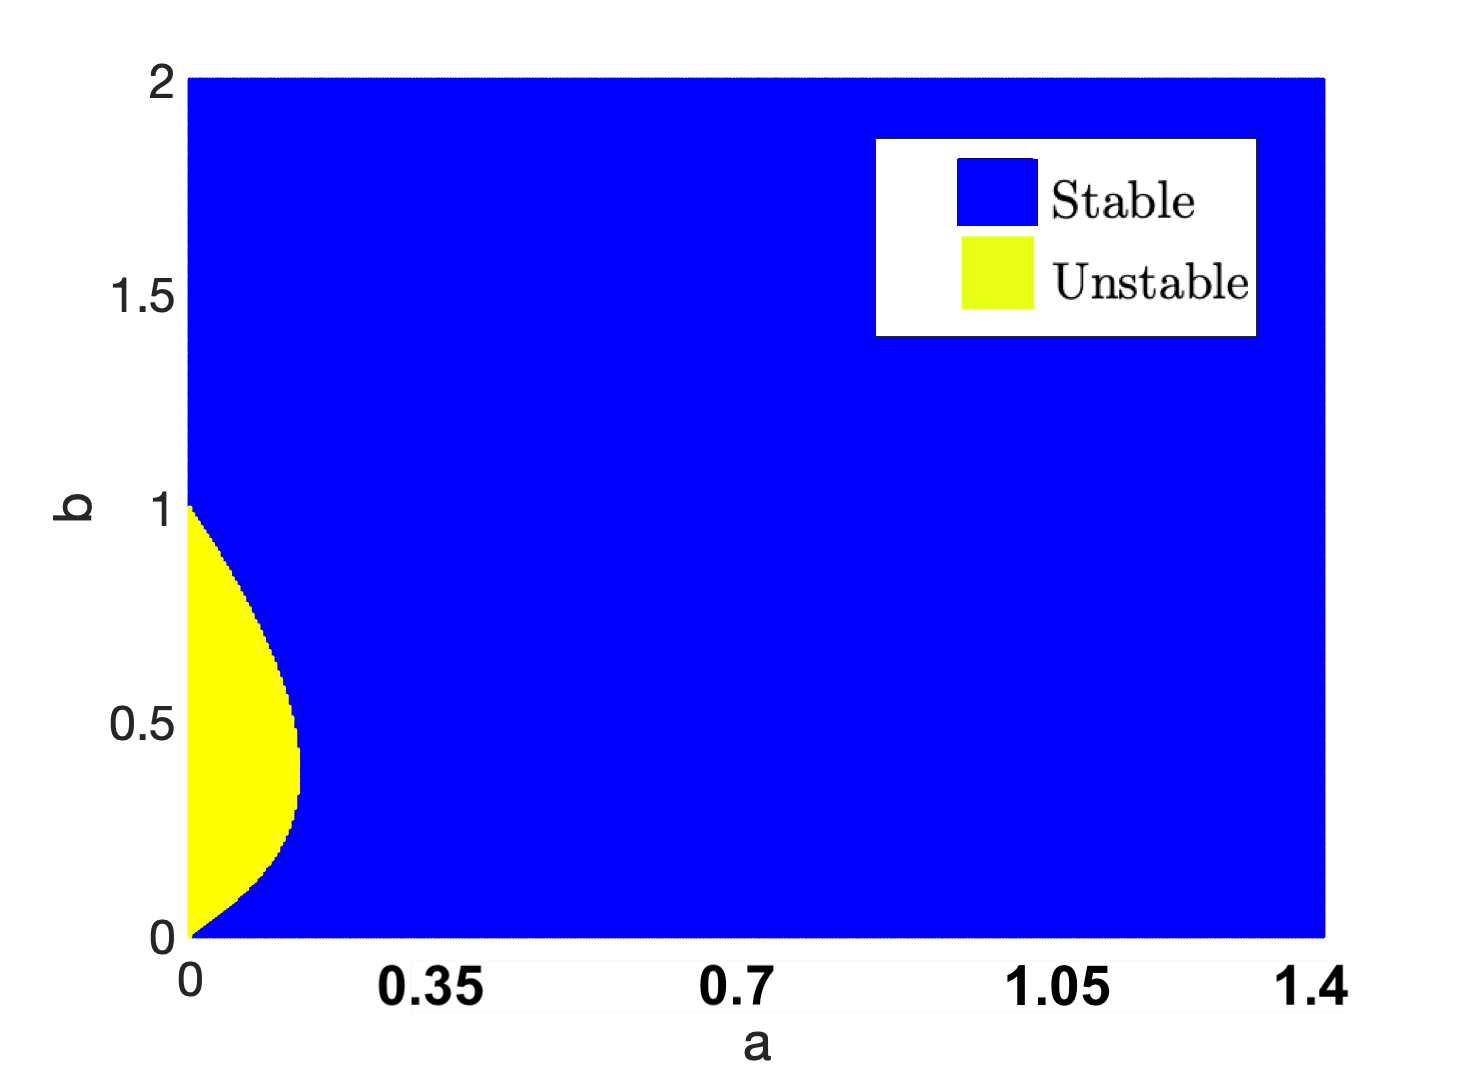
\includegraphics[width=8cm,height = 6cm]{bifsh.png}
        \caption{Bifurcation diagram for spatially homogeneous model, no delay.}
        \label{fig:bifsh}
    \end{subfigure}
    \hfill
    \begin{subfigure}[b]{0.45\textwidth}
        \centering
        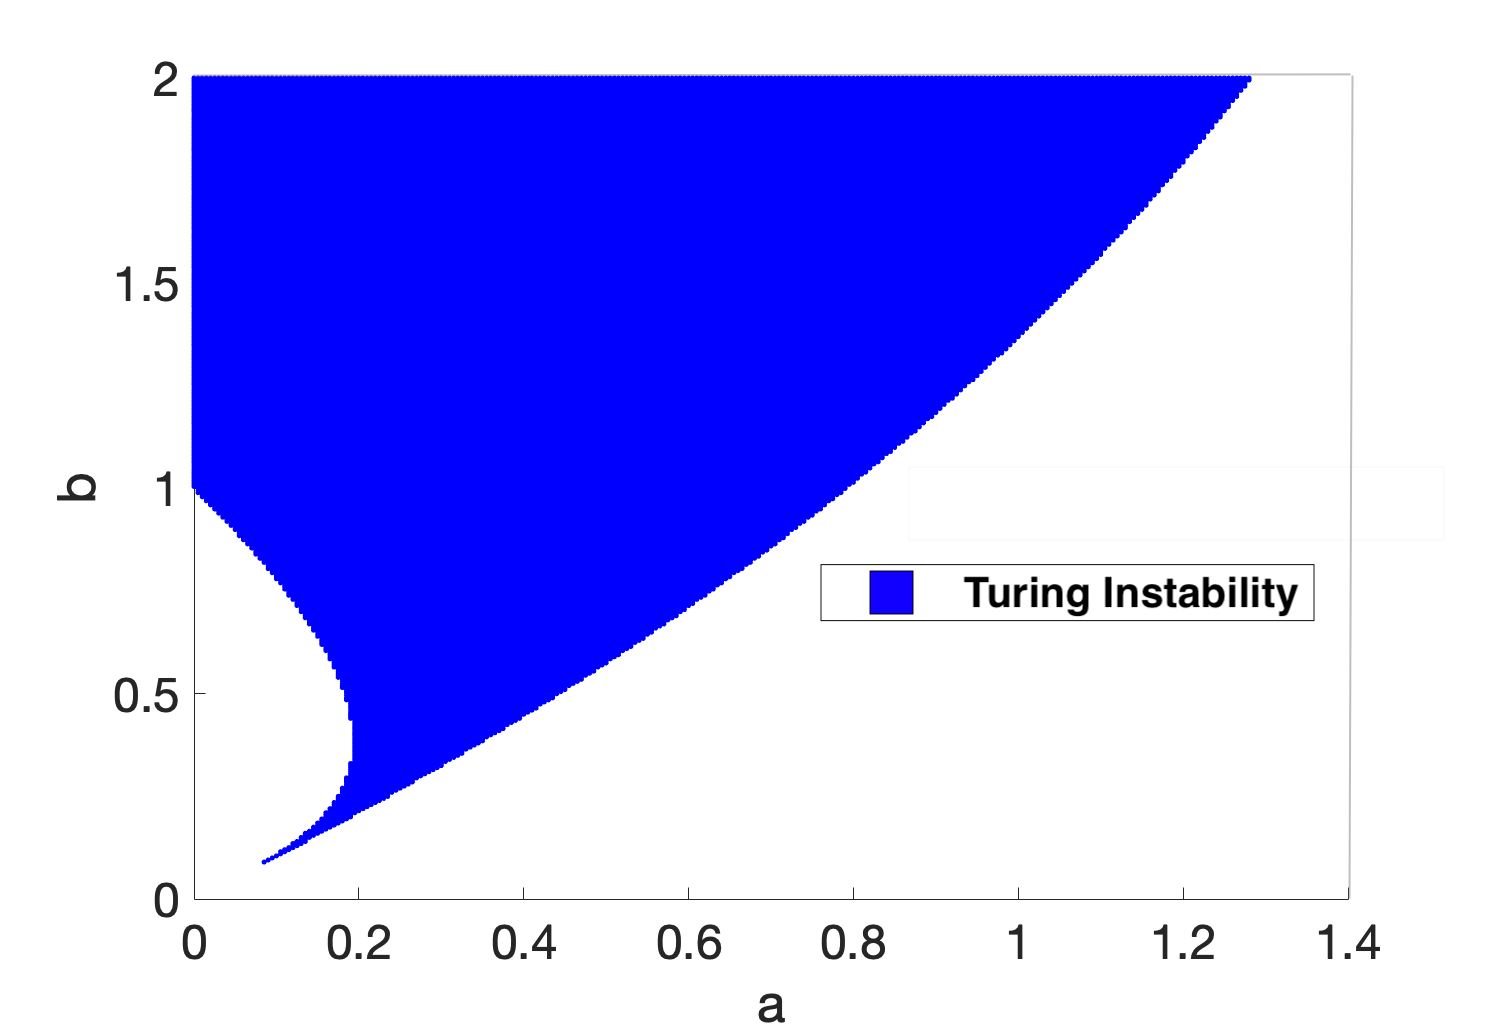
\includegraphics[width=8cm,height = 6cm]{turingspace.png}
        \caption{Turing space, no delay. $(\epsilon^2=0.001$.}
        \label{fig:turingspace}
    \end{subfigure}
    \caption{}
    \label{fig:dispfixed}
\end{figure}

\subsection{Numerical Implementation}\label{section:numimp}
\subsubsection{Spatial Discretisation}
In order to numerically resolve the spatial derivatives $\frac{\partial^2 u}{\partial x^2}$, $\frac{\partial^2 v}{\partial x^2}$ and implement the relevant boundary conditions, a finite-difference scheme is used. We use $m=500$ equally spaced spatial discretisation points on the domain $x\in\Omega=[0,1]$, with the spatially discretised points given as $\textbf{x}=[x_1,\cdots,x_m]^T$ where $x_i=(i-1)\Delta x$, with $\Delta x=\frac{1}{m-1}$. This ensures $x_1=0$ and $x_m=1$. Letting $U_i^t$ denote the numerical approximation to $u(x_i,t)$, we use a second-order central difference approximation \cite{finitediff} to evaluate the second-order derivatve $\frac{\partial^2 u}{\partial x^2}(x_i,t)$. Namely,
\begin{equation}
\frac{\partial^2 u}{\partial x^2}(x_i,t)\approx\frac{1}{\Delta x^2}\left(U_{i+1}^t-2U_i^t+U_{i-1}^t\right).
\end{equation}
By denoting $\textbf{U}^t$ as the vector of numerical approximations to $u(x,t)$ at some time $t$ across the whole spatial domain $\textbf{x}$, so that $\textbf{U}^t=\left[U_1^t,\cdots,U_m^t\right]^T$, the numerical approximation of the second-order derivative across the whole spatial domain at some time $t$ can be computed in matrix form as
\begin{equation}
    \frac{\partial^2 u}{\partial \textbf{x}^2}\approx A\textbf{U}^t.
\end{equation}
$A$ is the discrete second-order differential operator, and is given by
\begin{equation}\label{A}
A=\frac{1}{\Delta x^2}\begin{bmatrix}
   -2&  1&  &  & 0\\
   1&  -2&  1&  & \\
   &  \ddots&  \ddots&  \ddots& \\
   &  &  1&  -2& 1\\
   0&  &  &  1& -2
  \end{bmatrix}.
\end{equation}
The sparse nature of $A$ allows for computational advantages when implementing the finite-difference scheme. In order to implement homogeneous Neumann boundary conditions, a first-order central difference approximation is used with `ghost' nodes appended at $x_{-1}$ and $x_{m+1}$. This results in altering entries $A_{1,2}$ and $A_{m,m-1}$ from a $1$ to a $2$, as seen in \eqref{Aneumann}. Further details on using `ghost' nodes can be found in appenix \ref{appendix:extramath}. To implement homogeneous Dirichlet conditions, the first and last rows of $A$ are set to $0$, as seen in \eqref{Adirichlet}. Since homogeneous Dirichlet conditions require $u(x)=0$ at $x=0,1$ for all $t>0$, we also set the initial conditions and kinetic functions to equal $0$ at the end nodes.
\begin{multicols}{2}
\begin{equation}\label{Aneumann}
    \begin{split}
A&=\frac{1}{\Delta x^2}\begin{bmatrix}
   -2&  2&  &  & 0\\
   1&  -2&  1&  & \\
   &  \ddots&  \ddots&  \ddots& \\
   &  &  1&  -2& 1\\
   0&  &  &  2& -2
  \end{bmatrix}.\\
  A &\textit{ with homogeneous Neumann conditions}
    \end{split}
\end{equation}
\break
\begin{equation}\label{Adirichlet}
    \begin{split}
A&=\frac{1}{\Delta x^2}\begin{bmatrix}
   -0&  0& \cdots &  & 0\\
   1&  -2&  1&  & \\
   &  \ddots&  \ddots&  \ddots& \\
   &  &  1&  -2& 1\\
   0&\cdots  &  &  0& 0
  \end{bmatrix}.\\
  A & \textit{ with homogeneous Dirichlet conditions}
    \end{split}
\end{equation}
\end{multicols}

\subsubsection{Temporal Discretisation}
